\documentclass{article}
\usepackage[catalan]{babel}
\usepackage[a4paper, total={6.5in, 9.5in}]{geometry}
\usepackage{multirow}
\usepackage{graphicx}

\begin{document}

\nocite{*}

\title{\textbf{Implementació d'un Sistema RISC-V en \textit{FPGA} amb suport per \textit{Linux}} \\
Informe de seguiment II}
\author{Oscar Lostes Cazorla}
\date{Desembre 2021}

\clearpage\maketitle
\thispagestyle{empty}

\newpage

\section{Comparativa d'objectius respecte a l'informe de seguiment anterior}

A l'anterior informe es van exposar les següents fites a curt termini:
\begin{itemize}
\item Determinar si el \textit{SoC} per defecte compleix els requisits de recursos com per a cabre a les nostres plaques, i fer els canvis de configuració necessaris si s'escau.
\item Creació del component \textit{Qsys} a partir del \textit{SoC}.
\item Integració del \textit{SoC} amb la resta de dispositius del sistema.
\item Programació efectiva de la \textit{FPGA}, on el sistema fos capaç d'executar algun software (encara que sigui \textit{baremetal} directament des de la BootROM)
\end{itemize}

D'aquests objectius, només s'han aconseguit de forma efectiva els 2 primers, ja que la integració del \textit{SoC} està comportant alguns problemes.

\subsection{Configuració i ús de recursos del \textit{SoC}} \label{config}

Després de les primeres proves de síntesi a partir de la generació per defecte del \textit{RockeChip}, s'observa un ús desmesurat de recursos \textit{LE (Logic Elements)} (de l'ordre del 300\%).
Una anàlisi de l'ús individualitzat dels recursos per cada component del disseny revela que els components amb més contribució eren les memòries \textit{cache} (tant de primer com de segon nivell).
Aquesta observació es confirma experimentalment amb l'eliminació de la \textit{cache} L2 i la reducció al mínim de la \textit{cache} L1 (ja que \textit{Chipyard} no permet eliminar fàcilment l'L1). Aquests canvis de configuració porten el disseny a unes dimensions acceptables (de l'ordre del 70\%).
\\

Tot i això, aquesta solució dista de ser òptima i no explica per què les memòries disparen tant les dimensions del disseny.
Després d'analitzar el codi Verilog generat per \textit{Chipyard}, així com consultant la documentació, s'arriba a la conclusió que les memòries del disseny no s'estan reconeixent com a tal: \textit{Quartus} està intentant sintetitzar aquests mòduls Verilog a partir d'una descripció comportamental, que no permet que l'eina infereixi que es tracten de memòries, i, per tant, en fa una síntesi literal amb lògica.
Això es tradueix en memòries que utilitzen gran quantitat de recursos, ignorant els blocs de memòria disponibles a la \textit{FPGA}.
\\

Preguntant a la \textit{mailing list} del projecte, es conclou que el mètode de generació emprat no és l'adeqüat pel cas d'ús, i es troba l'alternativa correcta. Amb aquest \textit{workflow} de generació, la resta de components es mantenen pràcticament inalterats, mentre que les memòries es generen amb descripcions de \textit{flip-flops} que \textit{Quartus} pot inferir com a memòries correctament.
Això resulta en un disseny amb dimensions acceptables (de l'ordre del 50\%), fins i tot després d'haver reactivat l'L2 i retornat l'L1 a quantitats raonables, ja que ara les \textit{caches} fan servir recursos de memòria (inferior al 10\%) en comptes de \textit{LEs}.
\\

Les característiques més importants de la configuració actual (que probablement no serà la definitiva) són:
\begin{itemize}
\item 1 RocketCore gran (versió amb totes les capacitats)
\item \textit{Cache} L1 associativa de 1 \textit{Kib} i 2 vies (una de dades, i una altra d'instruccions)
\item \textit{Cache} L2 associativa de 512 \textit{KiB} i 8 vies
\item Un únic port extern (\textit{AXI4}, en aquest cas): el de memòria.
\end{itemize}

\subsection{Component \textit{Qsys}}

Importar el codi Verilog al dissenyador de plataformes de \textit{Quartus} ha estat un procés bastant directe: indicar els arxius Verilog involucrats en el disseny, seleccionar la \textit{top-level entity} (\textit{ChipTop}, en aquest cas) i obtenir el component. Després, aquest component es pot portar a \textit{Quartus} sense gaire dificultat i obtenir una síntesi correcta.
\\

Cal destacar una part del procés, que no ha estat tan directa: la generació de les interfícies del component. \textit{Qsys} intenta inferir automàticament les interfícies a partir d'un estàndard de noms dels senyals del mòdul del qual es genera el component. \textit{Chipyard} no utilitza aquests noms estàndard, i, per tant, aquesta inferència falla, obtenint interfícies incorrectes. Per tant, s'han de re-mapejar els senyals manualment.

\subsection{Integració del \textit{SoC}}

Obtenir un component \textit{Qsys} amb el \textit{SoC} no és suficient per a tenir el sistema complet. Al voltant d'aquest component s'hi han de connectar una sèrie d'elements externs.
El primer que s'intenta integrar (i probablement el més important) és la memòria principal \textit{RAM} del sistema.
\\

Aquesta tasca, al contrari que la generació del component \textit{Qsys}, està resultant problemàtica i és l'actual escull pel progrés del projecte.
Unes quantes de les plaques \textit{FPGA} de les que es disposa pel projecte ofereixen accés a memòries SDRAM integrades. Idealment, es vol emprar aquests dispositius com a memòria principal del sistema (en comptes d'emprar recursos de memòria interna de la \textit{FPGA}, com es fa amb les \textit{caches}).
El problema és que les plaques que disposen d'aquestes memòries també disposen d'un processador integrat, para\lgem elament amb la \textit{FPGA} (\textit{HPS, Hard Processor System}), i la memòria es troba connectada directament amb aquest HPS.
\\

Per defecte, no es pot accedir als recursos del \textit{HPS} des de la \textit{FPGA}. Per a poder utilitzar aquests recursos, s'ha d'utilitzar el component \textit{Qsys} corresponent al \textit{HPS}. Normalment, aquest component s'usa quan es farà ús directe del \textit{HPS}, però també permet configurar la cessió de recursos per a la \textit{FPGA}. Amb aquest component, podem obrir (entre d'altres) l'accés a la \textit{RAM} des de la \textit{FPGA}.

\begin{figure}[h]
\centering
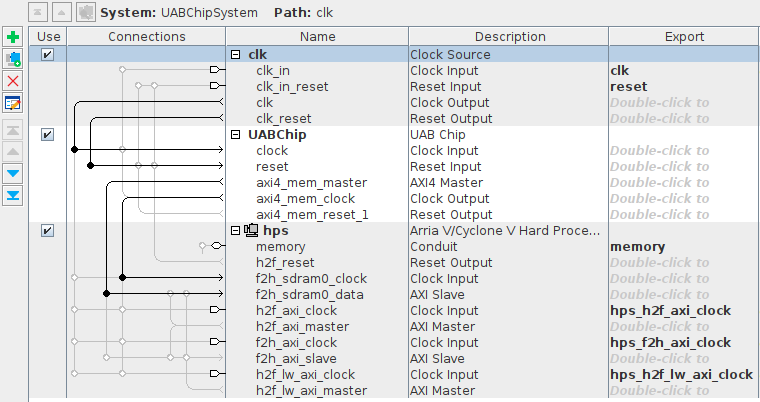
\includegraphics[width=15cm]{Qsys.png}
\caption{Projecte de \texttt{Qsys}}
\label{fig:qsys}
\end{figure}

Si bé semblaria que això hauria de ser suficient, el sistema resultant no és sintetitzable. S'ha trobat un exemple de projecte proporcionat per \textit{Terasic}, on queda clar que s'han de fer servir més components i algunes configuracions addicionals. Ara bé, encara no s'ha intentat integrar aquest exemple amb el projecte, i està com a tasca pendent.

\section{Següents passos}

D'acord amb els punts exposats a l'informe, s'actualitza la llista de fites a curt termini:
\begin{itemize}
\item Configurar l'accés a la \textit{SDRAM} des de la \textit{FPGA}
\item Programació efectiva de la \textit{FPGA}, on el sistema sigui capaç d'executar algun software (es proposa un programa \textit{baremetal} que encengui els \textit{LEDs} de la placa)
\item Configurar l'accés a la resta de perifèrics (\textit{UART} i \textit{SD}, com a mínim) des de la \textit{FPGA}
\end{itemize}

Si s'aconsegueixen aquestes fites, es podrà passar de forma efectiva a la següent fase del projecte, on s'intenti executar \textit{Ubuntu} sobre aquest sistema, tal com es va plantejar a l'informe anterior.

\end{document}
